\documentclass[newPxFont,sthlmFooter]{beamer}
\usetheme{sthlm}
\usepackage[utf8]{inputenc}
\usepackage{booktabs}
\usepackage{multirow}
\usepackage{hyperref,graphicx}
\usepackage{fourier-orns}
\usepackage[LGRgreek]{mathastext} % For Non-ilatized math equations
\usepackage{chronology}
\usepackage{fontawesome}
\usepackage{hyperref}
\usepackage{appendixnumberbeamer}
\hypersetup{pdfpagemode=FullScreen}
\renewcommand{\event}[3][e]{%
  \pgfmathsetlength\xstop{(#2-\theyearstart)*\unit}%
  \ifx #1e%
    \draw[fill=black,draw=none,opacity=0.5]%
      (\xstop, 0) circle (.2\unit)%
      node[opacity=1,rotate=45,right=.2\unit] {#3};%
  \else%
    \pgfmathsetlength\xstart{(#1-\theyearstart)*\unit}%
    \draw[fill=black,draw=none,opacity=0.5,rounded corners=.1\unit]%
      (\xstart,-.1\unit) rectangle%
      node[opacity=1,rotate=45,right=.2\unit] {#3} (\xstop,.1\unit);%
  \fi}%
\newcommand{\fs}{\footnotesize}
\newcommand{\scs}{\scriptsize}
\newcommand{\ty}{\tiny}
%%%%%%%%%%%%%%%%%%%%%%%%%%%%%%%%%%%%%%%%%%%%%%%%%%%%%%%%%%%%%%%%%%%%%%%%%%%%%%%%%%%%%%%%%%%

\title{\vspace{1cm}\LARGE Road to Research Writing: \vspace{-0.2cm}}
\subtitle{\Large Brief Summary on Methods and Tools}
\date{}
\author{{\textcolor{orange}{
\footnotesize \bf Dr. P. A. Praveen}}\\\footnotesize {Post-Doctoral Fellow \\ {\it Indian Institute of Science Education \& Research,\\ Tirupati, Andhra Pradesh}\vspace{0.2cm}\\ \faEnvelope~~~\texttt{contact@prvn.info}} }
\institute{\footnotesize {\bf June 04, 2021} \vspace{0.5cm} \\
\href{http://prvn.info}{
\includegraphics{figs/doi.png}} \vspace{-0.5cm}}

%%%%%%%%%%%%%%%%%%%%%%%%%%%%%%%%%%%%%%%%%%%%%%%%%%%%%%%%%%%%%%%%%%%%%%%%%%%%%%%%%%%%%%%%%%%%%

\begin{document}
{\usebackgroundtemplate{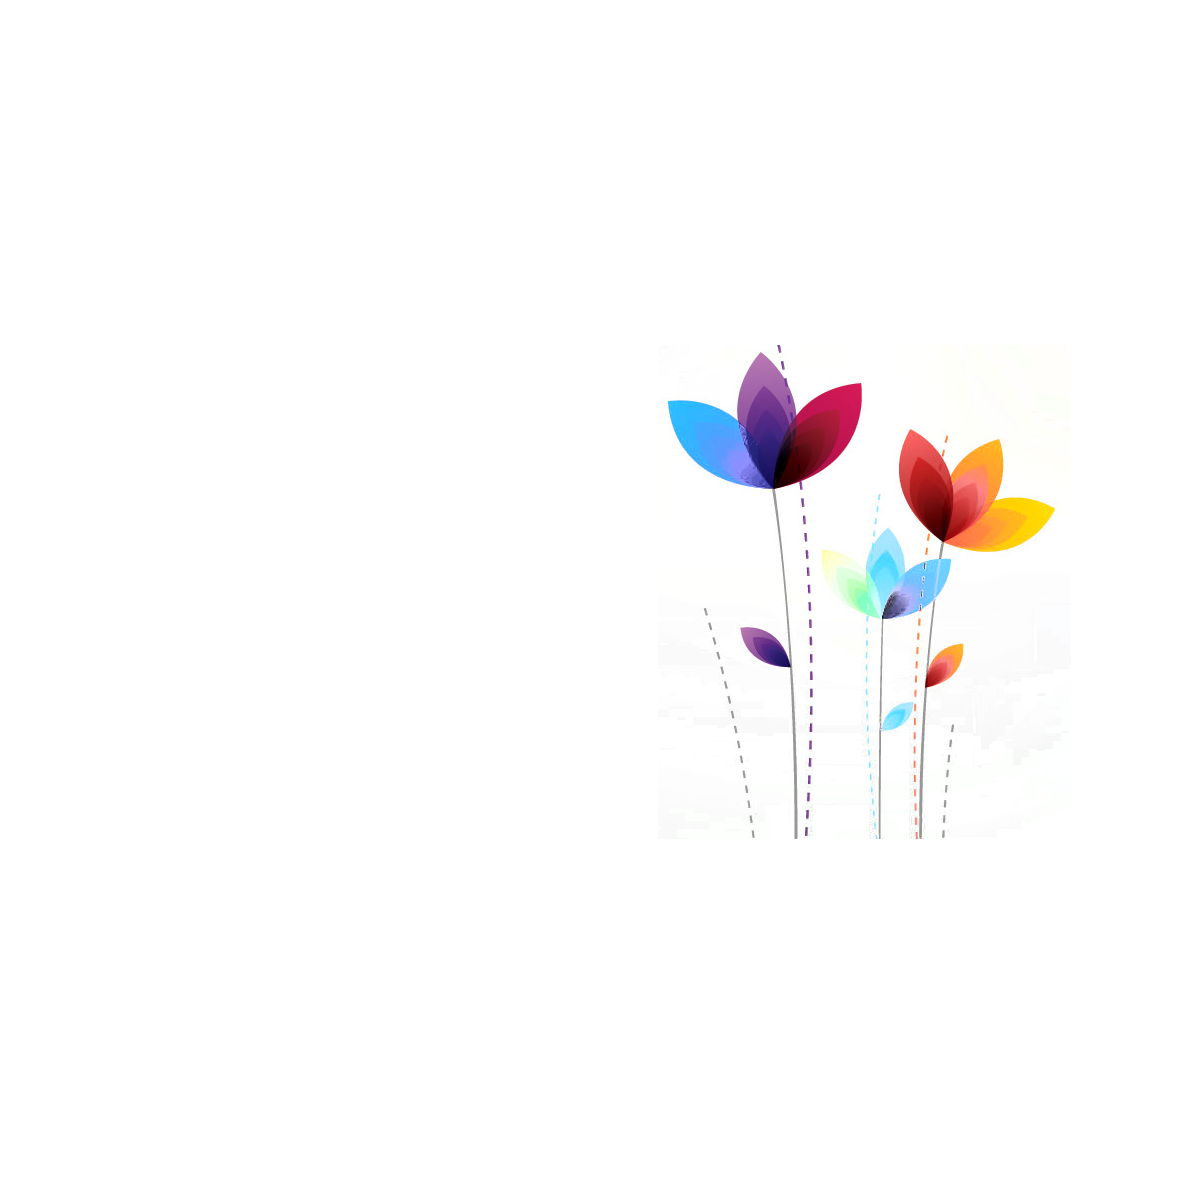
\includegraphics[width=5.5in]{figs/bg-2.png}}%
\maketitle
}

\begingroup
\setbeamercolor{background canvas}{bg=sthlmDarkGrey}
\begin{frame}[plain,containsverbatim]
\begin{figure}
\centering
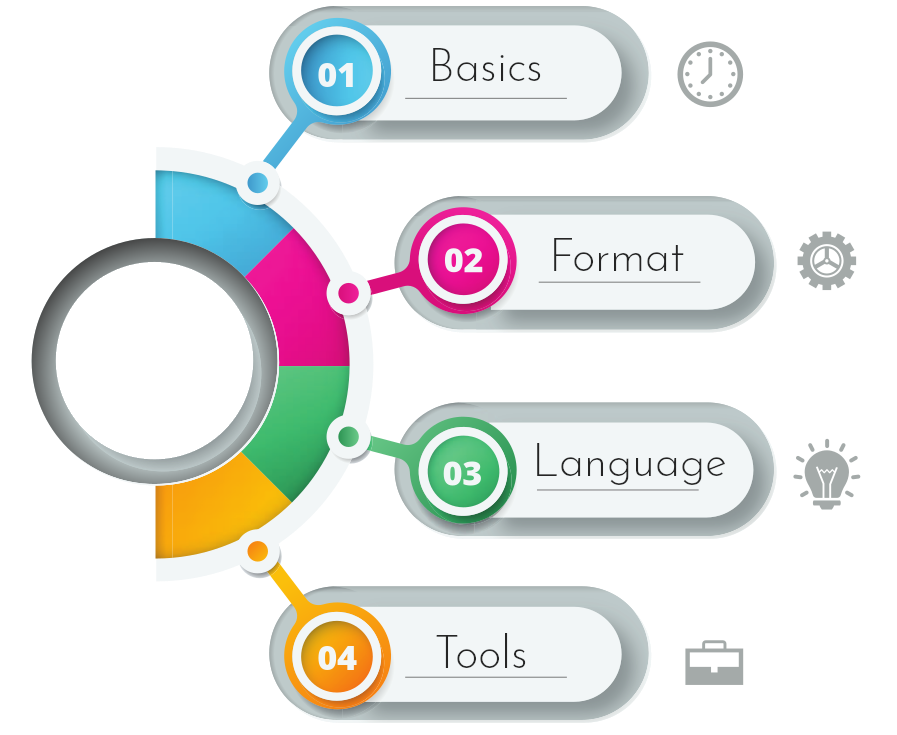
\includegraphics[width=3in]{figs/plan}
\end{figure}
\end{frame}
\endgroup

\section{Part 1: Basics}

\begin{frame}\frametitle{Ethics in scientific communication}
  \begin{columns}[T,onlytextwidth]
    \column{0.5\textwidth}
  \begin{figure}
    \centering
    
\includegraphics[width=2in]{figs/eth} 
  \end{figure}
    \column{0.5\textwidth}
      \vspace{1cm}
  \begin{itemize}
  \fs
    \item Scientific research crucially depends on the integrity of the investigators
    \item Fabrication and falsification clearly are unethical
    \item The publication should be complete
    \item Should support the advancement of science
  \end{itemize}
  \vspace{-2cm}
  \end{columns}
\end{frame}

\begin{frame}\frametitle{When and what to publish}
  \begin{columns}[T,onlytextwidth]
    \column{0.5\textwidth}
  \begin{figure}
    \centering
    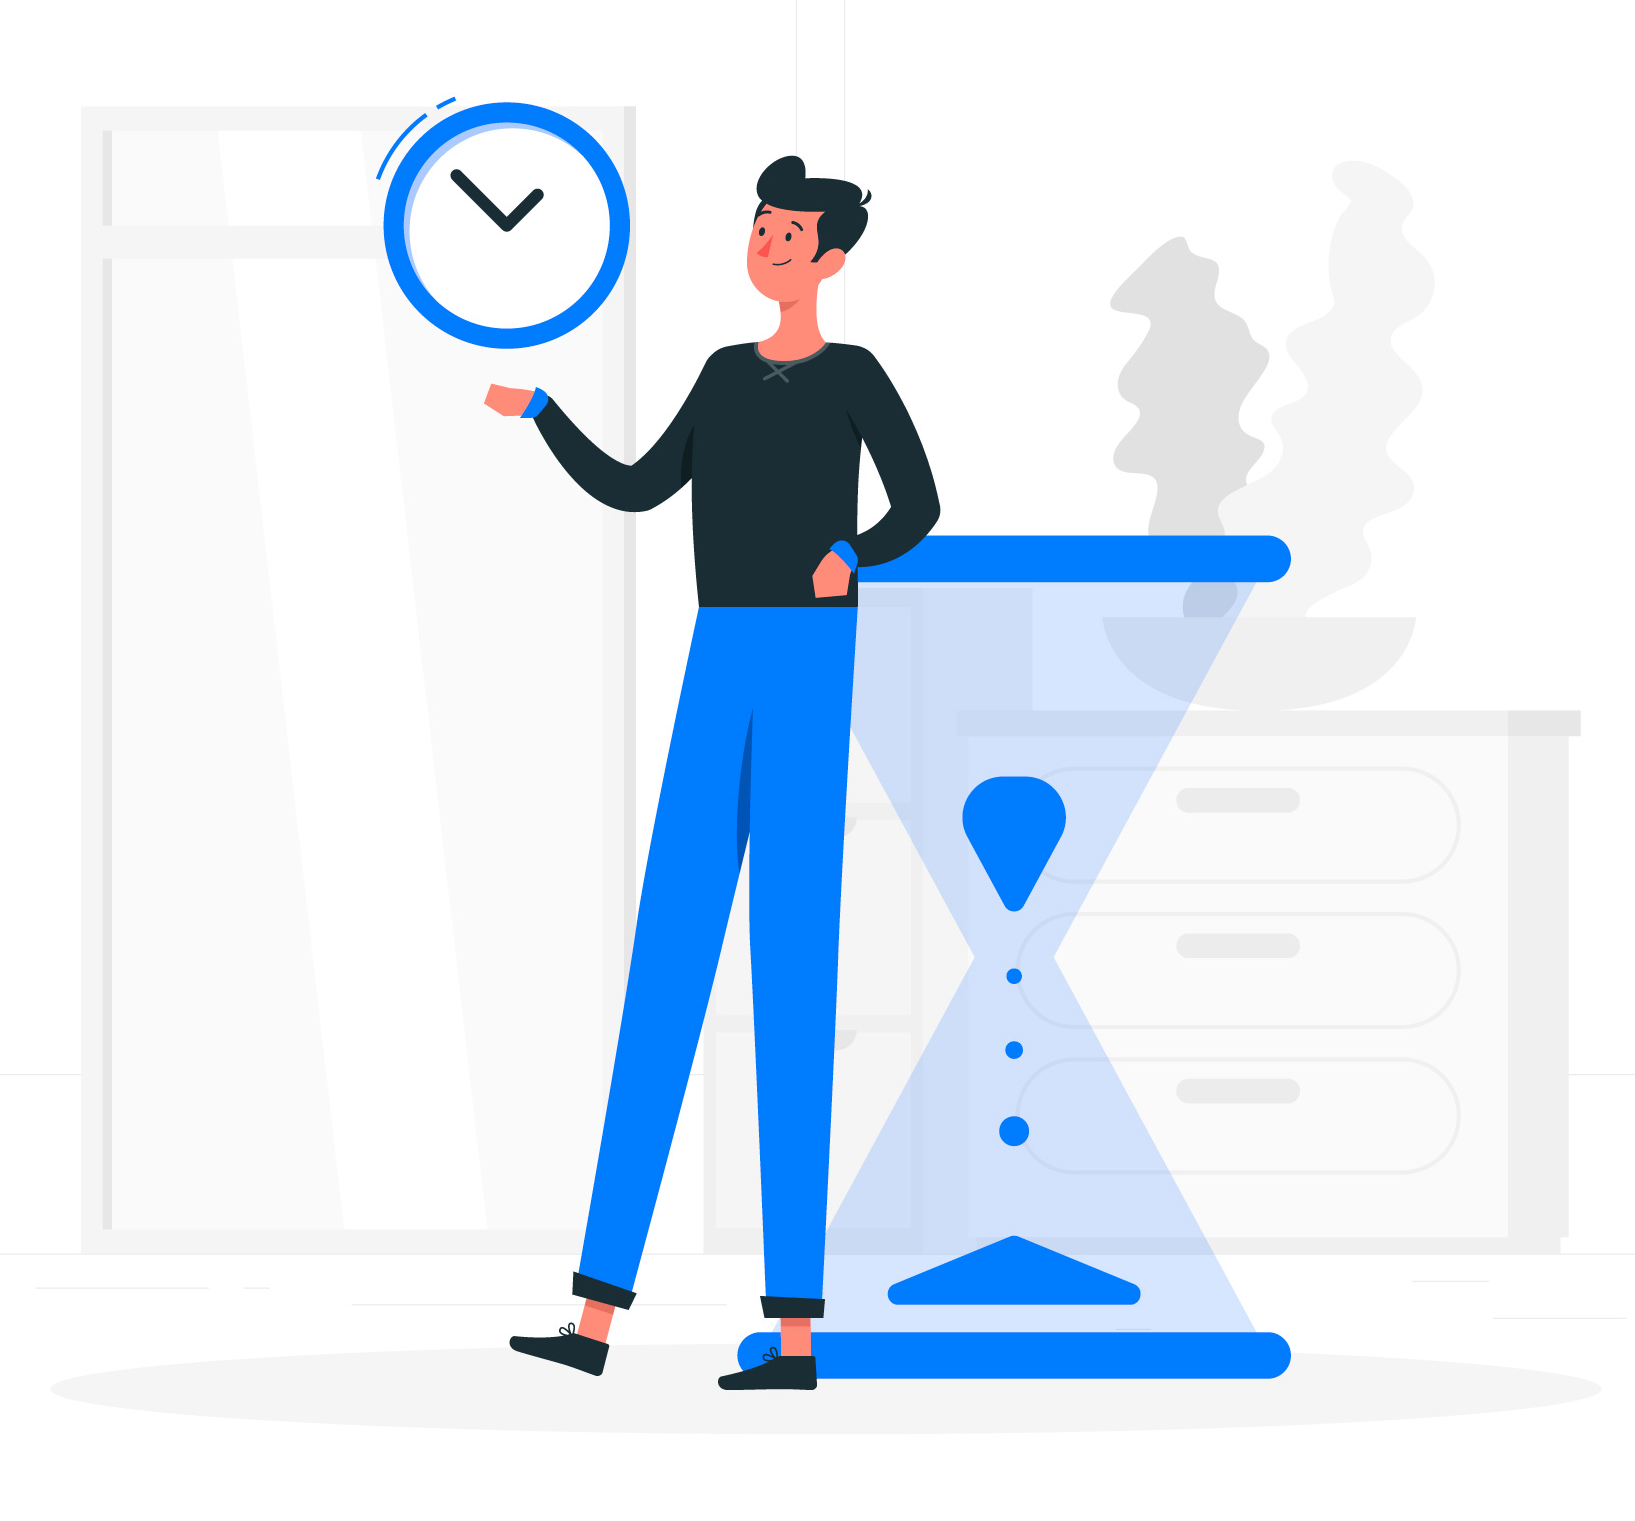
\includegraphics[width=2in]{figs/time} 
  \end{figure}
    \column{0.5\textwidth}
      \vspace{1cm}
  \begin{itemize}
  \fs
    \item Not too early; Not too late
    \item Enough work with enough results
    \item Results lead to clear understanding
    \item Avoid short, incomplete descriptions
    \item Don't fall for `publish or perish'
  \end{itemize}
  \vspace{-2cm}
  \end{columns}
\end{frame}

\begin{frame}\frametitle{Don't be a prey!}
\begin{block}{\small Always remember this:}
\footnotesize
\begin{itemize}
\item Reputation of an investigator is determined by the quality of research done over an extended time
\item Large number of low-quality publications is not of benefit to the individual or the profession
\item Don't tempted to publish the same material, or material only slightly different, multiple times
\end{itemize}
\end{block}
\begin{figure}
    \centering
    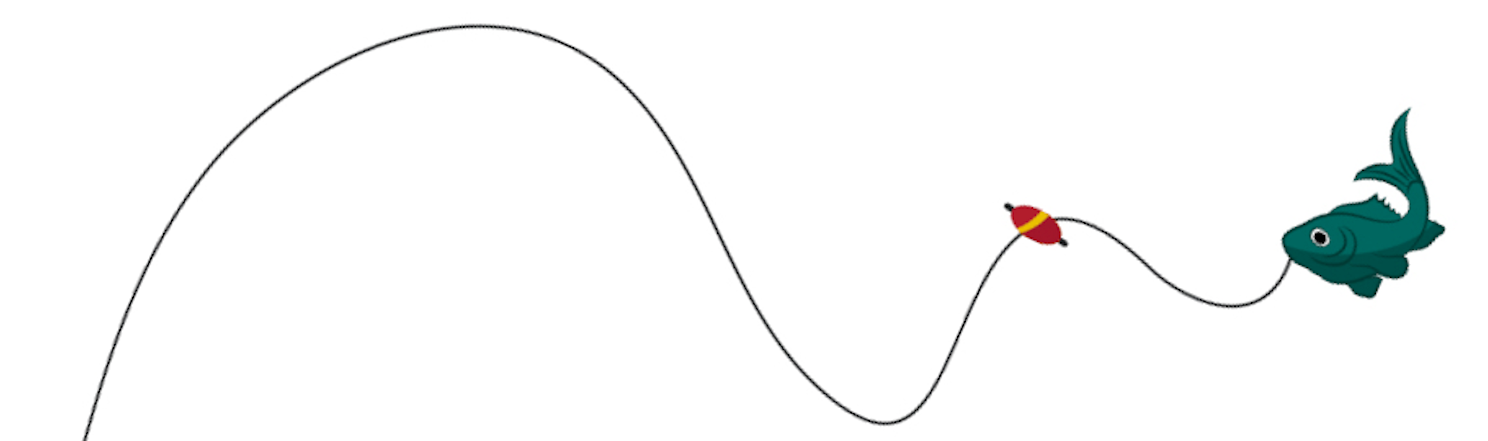
\includegraphics[width=2in]{figs/prey} 
  \end{figure}
\end{frame}

\begin{frame}\frametitle{Who are authors}
  \begin{columns}[T,onlytextwidth]
    \column{0.5\textwidth}
  \begin{figure}
    \centering
    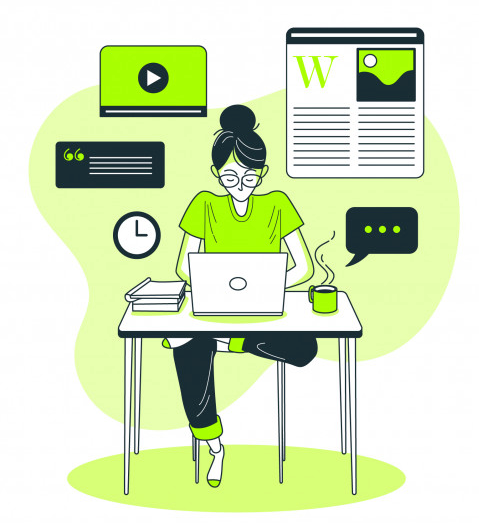
\includegraphics[width=2in]{figs/auth} 
  \end{figure}
    \column{0.5\textwidth}
%      \vspace{1cm}
  \begin{itemize}
  \fs
    \item Colleague prepared buffers or did routine computer programming \textcolor{red}{are not sufficient}
    \item \textcolor{red}{Extending research facility} can't be a contribution
    \item People who made \textcolor{teal}{significant and substantial intellectual contributions}
    \item The first author is assumed to have made the major contribution to the work
    \item Often supervisior is designated with corresponding author at the end
  \end{itemize}
  \vspace{-2cm}
  \end{columns}
\end{frame}

\begin{frame}\frametitle{Author contribution statement}
  \vspace{-0.5cm}
  \begin{itemize}
    \fs
  \item \textcolor{blue}{intention of recognizing individual author contribution}, reducing disputes and facilitating collaboration
  \item \textcolor{blue}{opportunity to share an accurate and detailed description} of their diverse contributions
  \item \textcolor{blue}{corresponding author is responsible} for ensuring that the descriptions are accurate and agreed by all authors
  \item \textcolor{blue}{role(s) of all authors should be listed,} using the relevant categories
  \end{itemize}
{\tiny{\bf Categories:} Conceptualization; Methodology; Software; Validation; Formal analysis; Investigation; Resources; Data Curation; Writing - Original Draft; Writing - Review \& Editing; Visualization; Supervision; Project administration}
\end{frame}

\begin{frame}\frametitle{Plagiarism}
{\bf Definition:} Act of presenting words, ideas, images, sounds or other creative expressions without proper attribution.
\begin{block}{\small What is plagiarism?}
\footnotesize
\begin{itemize}
\item \faClone~~{\bf Clone:} Submitting someone else's work as your own
\item \faCopy~~{\bf Ctrl-C:} Taking large portions of text from a source without alteration
\item \faRetweet~~{\bf Find \& Replace:} Changing key words and pharses but keeping essential content
\item \faRefresh~~{\bf Remix:} Paraphrasing from several sources
\item \faRecycle~~{\bf Recycle:} Borrowing from your own work (self-plagiarism)
\end{itemize}
\end{block}
%\begin{figure}
%    \centering
%    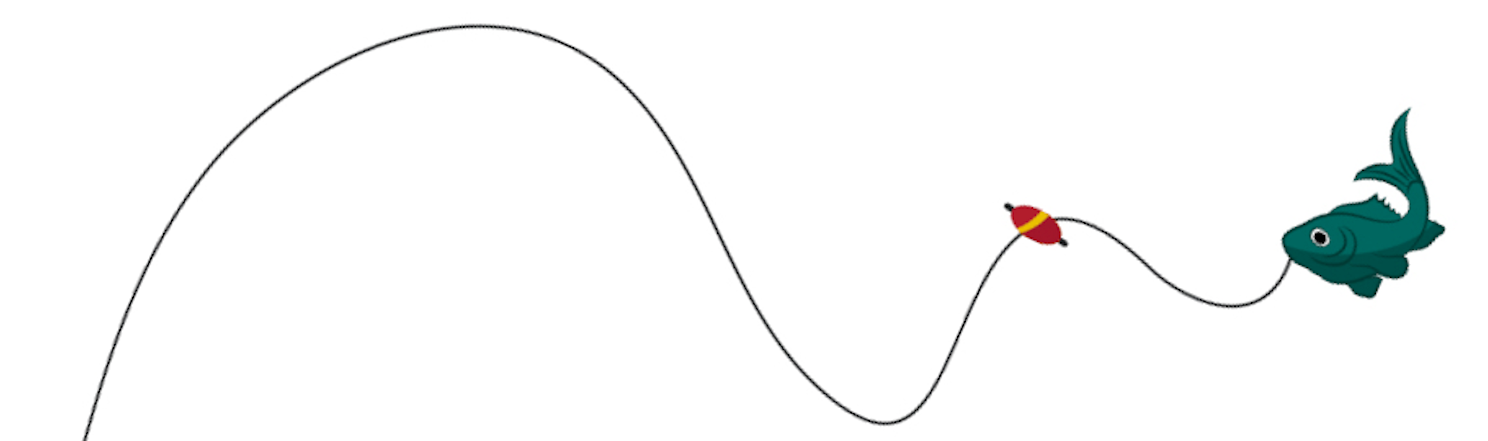
\includegraphics[width=2in]{figs/prey} 
%  \end{figure}
\end{frame}

\section{Part 2: Formating}

\begin{frame}\frametitle{Types of Books}

    \begin{columns}[T,onlytextwidth]
      \column{0.5\textwidth}
    \begin{figure}
      \centering
      
\includegraphics[width=2in]{figs/book} 
    \end{figure}
      \column{0.5\textwidth}
        \vspace{1cm}
    \begin{itemize}
    \fs
      \item \textcolor{orange}{\bf Proceeding volumes:} book based on meetings/conferences
      \item \textcolor{orange}{\bf Monograph:} books that examine a single topic in detail
      \item \textcolor{orange}{\bf Handbook:} large, multiauthored volumes that discuss a field in depth
    \end{itemize}
    \vspace{-2cm}
    \end{columns}
  \end{frame}
  
  \begin{frame}\frametitle{Types of journal presentations}
    \begin{columns}[T,onlytextwidth]
      \column{0.5\textwidth}
  %      \vspace{1cm}
    \begin{itemize}
      \fs
      \item \textcolor{purple}{\bf Articles:} provide important new data and fresh approach to an established subject
      \item \textcolor{purple}{\bf Notes:} preliminary reports of special significance
      \item \textcolor{purple}{\bf Communications:} (or letters) - preliminary reports of special significance and urgency subjected length restriction
      \item \textcolor{purple}{\bf Reviews:} integrate, correlate, and evaluate results from published literature on a particular subject
    \end{itemize}
    \column{0.5\textwidth}
          \vspace{0.5cm}
    \begin{figure}
      \centering
      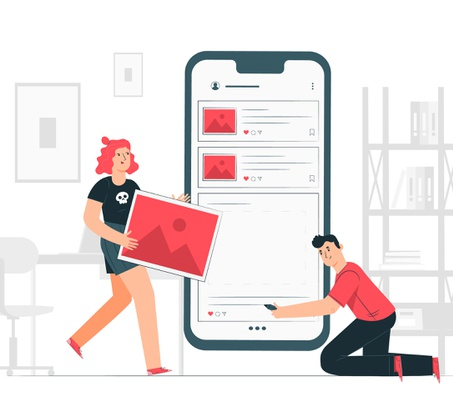
\includegraphics[width=2in]{figs/art} 
    \end{figure}
    \end{columns}
  \end{frame}
  
  \begin{frame}\frametitle{General structure}
    \begin{columns}[T,onlytextwidth]
      \column{0.5\textwidth}
    \begin{figure}
      \centering
      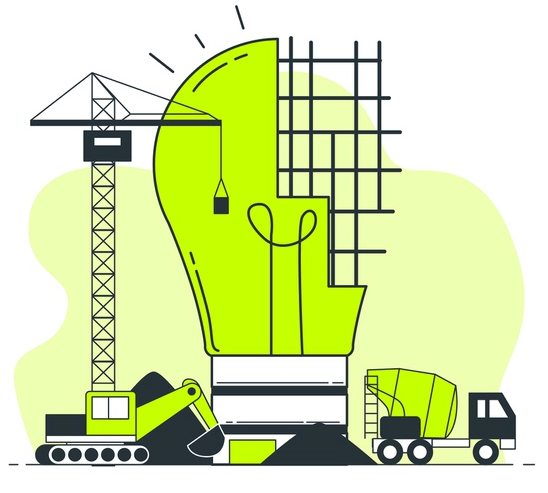
\includegraphics[width=2in]{figs/strc} 
    \end{figure}
      \column{0.5\textwidth}
  %      \vspace{1cm}
    \begin{itemize}
    \fs
      \item define the \textcolor{red}{problem}, create a \textcolor{teal}{hypothesis}, devise an experiment to \textcolor{blue}{test the hypothesis}, conduct the experiment, and draw \textcolor{purple}{conclusions}
      \item get a title that will reflect the paper's content and emphasis accurately and clearly within two lines
      \item extremely important step is to check the \textcolor{orange}{specific requirements of the publication} targeted and follow them
    \end{itemize}
    \vspace{-2cm}
    \end{columns}
  \end{frame}

\begin{frame}\frametitle{Manuscript structure}
  \vspace{-0.5cm}
  \begin{figure}
    \centering
    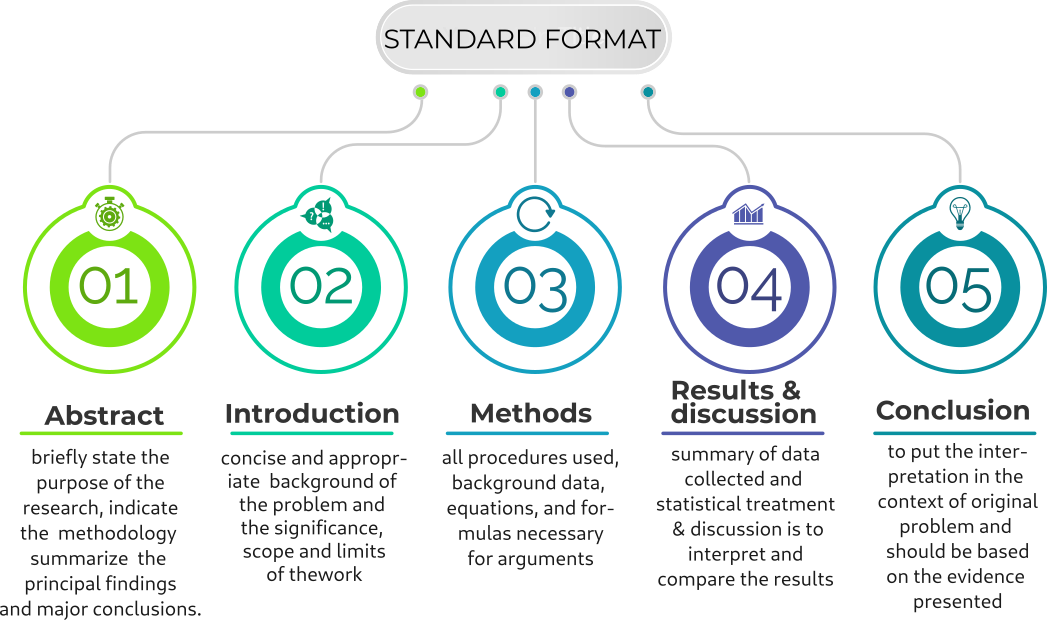
\includegraphics[width=4in]{figs/chart} 
  \end{figure}
\end{frame}

\begin{frame}\frametitle{Few more...}
  \vspace{-0.5cm}
  \begin{itemize}
    \fs
  \item \textcolor{blue}{\bf References:} proper attribution of the contributions of others by appropriate referencing - important ideas and experiments must be cited
  \item \textcolor{blue}{\bf Acknowledgements:} people who have assisted in the project, but not sufficiently for authorship, and to sponsoring agencies
  \item \textcolor{blue}{\bf Supporting info:} data relevant to advanced reader and supporting information
  \item \textcolor{blue}{\bf Rule of thumb:} all aspects of the research should be fully disclosed and reasonable assistance should be given to other researchers
  \end{itemize}
\end{frame}

\section{Part 3: Language}

\begin{frame}\frametitle{Sentence structure}
  \begin{columns}[T,onlytextwidth]
    \column{0.5\textwidth}
  \begin{figure}
    \centering
    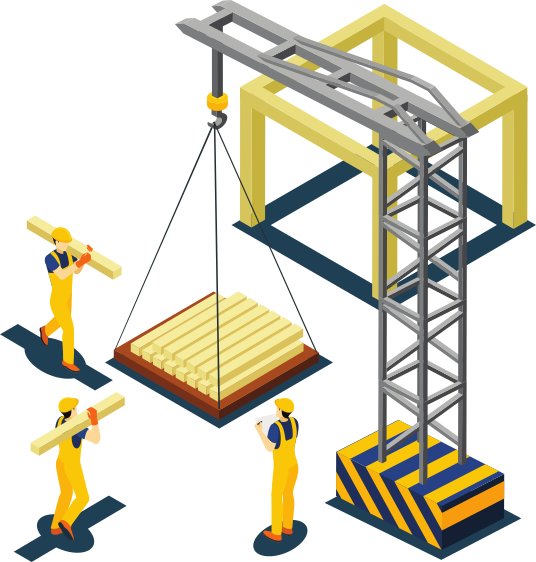
\includegraphics[width=2in]{figs/build} 
  \end{figure}
    \column{0.5\textwidth}
      \vspace{1cm}
  \begin{itemize}
  \fs
  \item short, simple declarative sentences
  \item sentences that make statements, rather than pose questions
  \item straight forward and easy to read
  \item avoid slang and jargon
  \end{itemize}
  \vspace{-2cm}
  \end{columns}
\end{frame}

{\usebackgroundtemplate{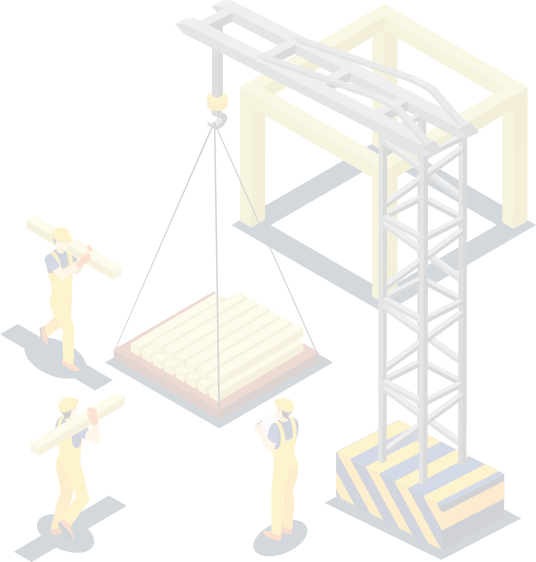
\includegraphics[width=4in]{figs/build-t}}
\begin{frame}\frametitle{Sentence structure}
  \begin{itemize}
  \fs
  \item Use the \textcolor{red}{active voice} when it is less wordy and more direct than the passive
  \item Use the \textcolor{red}{passive voice} when the doer of the action is unknown or not important or when you would prefer not to specify the doer of the action
  \item \textcolor{red}{Simple past tense} is correct for stating what was done, either by others or by you
  \item \textcolor{red}{Present tense} is correct for statements of fact
  \item \textcolor{red}{Present and simple past tenses} may both be correct for results, discussion, and conclusions
  \item Use \textcolor{red}{first person} when it helps to keep your meaning clear and to express a purpose or a decision
  \end{itemize}
\end{frame}}

\begin{frame}\frametitle{Key to right sentences}
  \begin{columns}[T,onlytextwidth]
    \column{0.5\textwidth}
  \begin{figure}
    \centering
    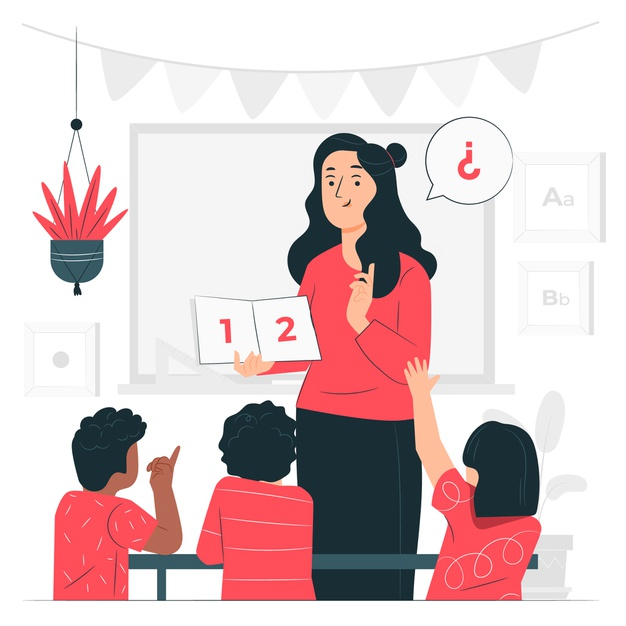
\includegraphics[width=2in]{figs/teach} 
  \end{figure}
    \column{0.5\textwidth}
      \vspace{1cm}
  \begin{itemize}
  \fs
  \item Be brief. Wordiness obscures your message and annoys your readers.
  \item Omit empty phrases
  \item Omit excess words
  \item Omit too much exaggeration
  \item Write economically (and usually more precisely)
  \end{itemize}
  \vspace{-2cm}
  \end{columns}
\end{frame}

\begin{frame}\frametitle{Gender neutral language}
  \begin{itemize}
  \fs
  \item Instead of \textcolor{red}{`man'}, use \textcolor{teal}{`people', `humans', `human beings', or `human species'}, depending on your meaning
  \item Instead of \textcolor{red}{`manpower'}, use \textcolor{teal}{`workers', `staff', `work force', `labor', `crew', `employees', or `personnel'}, depending on your meaning
  \item Instead of \textcolor{red}{`man-made'}, use \textcolor{teal}{`synthetic', `artificial', `built', `constructed', `manufactured', or even `factory-made'}
  \item Instead of \textcolor{red}{`he' and `his'}, change the construction to a plural form \textcolor{teal}{(`they' and `theirs')} or first person
  \item Using passive voice or second person \textcolor{teal}{(`you', `your', and `ours')} also works sometimes
  \item Instead of \textcolor{red}{`wife'}, use \textcolor{teal}{`family' or `spouse'} where appropriate
  \end{itemize}
\end{frame}

\begin{frame}\frametitle{Spacing}
  \begin{itemize}
  \fs
  \item Do not use square brackets, parentheses, or braces \textcolor{red}{around the symbol} for a quantity to make it represent any other quantity
  \item Use \textcolor{red}{italic type} for subscripts and superscripts that are themselves symbols for physical quantities or numbers
  \item Use \textcolor{red}{roman type} for subscripts and superscripts that are abbreviations and not symbols
  \item \textcolor{red}{Exponents} should follow subscripts
  \item \textcolor{red}{Use a slash (/)} in all subscript and superscript fractions, with no space on either side.
  \item \textcolor{red}{Leave no space around operators} in subscripts and superscripts
  \item \textcolor{red}{Leave no space around other expressions} in subscripts and superscripts, unless confusion or misreading would result
  \end{itemize}
\end{frame}

\begin{frame}\frametitle{Units}
  \begin{itemize}
  \fs
  \item Use \textcolor{blue}{metric and SI units} in all (possible) technical documents
  \item \textcolor{blue}{Abbreviate units} of measure when they accompany numbers
  \item Leave \textcolor{blue}{a space between} a number and its unit of measure
  \item Do not use a \textcolor{blue}{period after an abbreviated unit} of measure\\ (exception: in. for inch)
  \item Do not define units of measure
  \item Do not leave \textcolor{blue}{a space between} a number and the percent, angular degree, angular minute, or angular second symbols
  \item Use $^\circ$C with \textcolor{blue}{a space after a number}, but no space between the degree symbol and the capital C
  \item Do not add an 's' to make the \textcolor{blue}{plural of any abbreviated units of measure}. The abbreviations are used as both singular and plural
  \end{itemize}
\end{frame}

%%%

\begin{frame}\frametitle{Mathematical concepts}
  \begin{itemize}
  \fs
  \item \textcolor{blue}{Define all symbols} for first time you use them in the text
  \item Do not define \textcolor{blue}{standard mathematical constants} such as $\pi$ , $i$, and $e$
  \item Do not use an \textcolor{blue}{equal sign as an abbreviation} for the word `is' or the word `equals' in narrative text\\
	{\bf eg.} $PV = nRT$, where $P$ is pressure (not where $P = pressure$)
  \item Do not use a \textcolor{blue}{plus sign as an abbreviation} for the word `and' in narrative text\\
	{\bf eg.} a mixture of $A$ and $B$ (not a mixture of $A + B$)
  \item Do not use an \textcolor{blue}{asterisk to indicate multiplication} except in computer language expressions.
  
  \end{itemize}
\end{frame}

\begin{frame}\frametitle{Mathematical concepts (cont.)}
{\fs \bf Use italic type for:}\\
  \begin{itemize}
	\item \fs\textcolor{blue}{variables:} {\it T} for temperature, {\it x} for mole fraction, {\it r} for rate
	\item \fs\textcolor{blue}{axes:} the {\it y} axis
	\item \fs\textcolor{blue}{planes:} plane {\it P}
	\item \fs\textcolor{blue}{components of vectors and tensors:} ${\it a_1 + b_1}$
	\item \fs\textcolor{blue}{elements of determinants and matrices:} ${\it g_n}$
	\item \fs\textcolor{blue}{constants:} ${\it k_B}$, the Boltzmann constant; {\it g}, the acceleration due to gravity
	\item \fs\textcolor{blue}{functions that describe variables:} {\it f(x)}
  \end{itemize}
{\fs \bf Use boldface type for:}\\
  \begin{itemize}
  \fs
	\item \fs\textcolor{purple}{vectors}
	\item \fs\textcolor{purple}{tensors}
	\item \fs\textcolor{purple}{matrices} and
	\item \fs\textcolor{purple}{multidimensional physical quantities:} {\bf H}, magnetic field strength.
  \end{itemize}
\end{frame}

%%%

\begin{frame}\frametitle{Chemical names}
  \begin{columns}[T,onlytextwidth]
    \column{0.5\textwidth}
  \begin{figure}
    \centering
    
\includegraphics[width=2in]{figs/chem} 
  \end{figure}
    \column{0.5\textwidth}
      \vspace{0.3cm}
  \begin{itemize}
  \fs
  \item Greek locants, with no space after the comma
  \item Use hyphens to separate locants and configurational descriptors
  \item Do not use hyphens to separate the syllables of a chemical name unless the name is too long to fit on one line
  \item `Poly' is a syllabic prefix, not a descriptor, and no special treatment for that
  \end{itemize}
  \vspace{-2cm}
  \end{columns}
\end{frame}

\begin{frame}\frametitle{Citing references}
\begin{block}{\small Three common citing methods}
  \begin{itemize}
  \fs
  \item By {\bf superscript numbers}, which appear outside the punctuation if the citation applies to a whole sentence or clause
  \item By {\bf italic numbers} in parentheses on the line of text and inside the punctuation
  \item By {\bf author name and year of publication} in parentheses inside the punctuation (known as author-date)
  \end{itemize}
  \end{block}
\end{frame}

\begin{frame}\frametitle{Citing references}
  \begin{itemize}
  \fs
  \item If a reference has two authors, give both names \textcolor{blue}{joined by the word 'and'}
  \item If a reference has more than two authors, give only the first name listed, \textcolor{blue}{followed by 'et al.'}
  \item Do not use a \textcolor{blue}{comma before et al.}; always use a period \textcolor{blue}{after 'al.'}
  \item To cite more than one reference by the same principal author and various coauthors use the principal author’s name followed by \textcolor{blue}{'and co-workers' or 'and colleagues'}
  \item When citing more than one reference at one place by number in one of the numerical systems, \textcolor{blue}{list the numbers in ascending order} and separate them by commas
  \end{itemize}
\end{frame}

\begin{frame}\frametitle{Graph or Table?}
  \begin{columns}[T,onlytextwidth]
    \column{0.5\textwidth}
  \begin{figure}
    \centering
    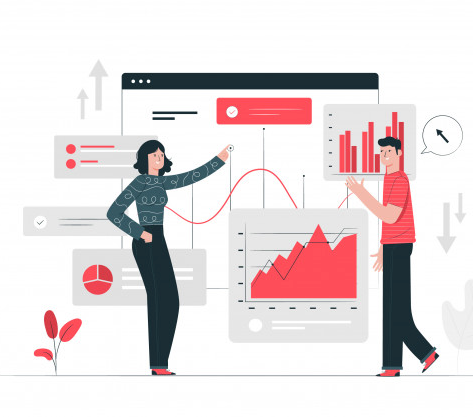
\includegraphics[width=2in]{figs/grap} 
  \end{figure}
    \column{0.5\textwidth}
%      \vspace{1cm}
  \begin{itemize}
  \fs
  \item \textcolor{blue}{\bf Use graphs}
	  \begin{itemize}
	    \fs
	  \item if basic point to be communicated at a glance
	  \item if reader to see trends and relationships
	  \end{itemize}
  \item \textcolor{teal}{\bf Use tables}
	    \begin{itemize}
	      \fs
	  \item if the reader to see exact numbers
	  \item if want to communicate a lot of information with words
	    \end{itemize}
%   \item Still undecissive? Check previous data representations
  \end{itemize}
  \vspace{-2cm}
  \end{columns}
\end{frame}

\begin{frame}\frametitle{Tables}
\begin{exampleblock}{\small When to use tables?}
  \begin{itemize}
  \fs
  \item when the data cannot be \textcolor{blue}{presented as narrative}
  \item when many \textcolor{blue}{precise numbers} must be presented
  \item when meaningful \textcolor{blue}{interrelationships} can be better conveyed
  \item tables \textcolor{blue}{should supplement, not duplicate,} text and figures.
  \end{itemize}
\end{exampleblock}

\begin{alertblock}{\small How to cite tables?}
  \begin{itemize}
  \fs
  \item \textcolor{red}{capitalize the word `Table'} when it is followed by the table number
  \item \textcolor{red}{number tables sequentially} with arabic or roman numerals
  \item \textcolor{red}{discuss tables sequentially} so that Table 1 is discussed before Table 2
  \end{itemize}
\end{alertblock}

\end{frame}

\begin{frame}\frametitle{Tables}
\vspace{-0.25cm}
\begin{block}{\small How to prepare tables?}
  \begin{itemize}
  \fs
  \item formal table should consist of \textcolor{purple}{at least three interrelated columns and three rows}
  \item if you have only \textcolor{purple}{two columns,} try writing the material as \textcolor{purple}{narrative}
  \item if the columns do not relate to each other \textcolor{purple}{use a list of items}
  \item if table has \textcolor{purple}{unusual requirements,} perhaps it should really be a figure
  \item tables should be \textcolor{purple}{simple and concise;} arrange all data for optimal use of space
  \item if you have many \textcolor{purple}{small tables, consider combining some}
  \item be \textcolor{purple}{consistent with symbols and abbreviations} among tables and between tables and text
  \item each table should have a \textcolor{purple}{concise title and appropriate column headings}
  \end{itemize}
\end{block}
\end{frame}

\begin{frame}\frametitle{Figures}
\vspace{-0.75cm}
\begin{exampleblock}{\small When to use figures?}
  \begin{itemize}
  \fs
  \item when the data can be \textcolor{blue}{highlighted, clarified and summarizing results}
  \item figures can be \textcolor{blue}{graphs of data, photographs, sketches, flow charts, etc.}
  \item \textcolor{teal}{line graphs} show trends. \textcolor{teal}{Bar graphs} compare magnitudes
  \item \textcolor{teal}{pie charts} show relative portions of a whole
  \item \textcolor{teal}{photographs} can provide absolute proof of findings
  \item \textcolor{blue}{excessive number of figures can dilute} the value of any individual figure
  \end{itemize}
\end{exampleblock}

\begin{alertblock}{\small How to cite figures?}
  \begin{itemize}
  \fs
  \item \textcolor{red}{capitalize the word `Figure'} when it is followed by the table number
  \item \textcolor{red}{number figures sequentially} with arabic numerals
  \item parts of the figure can be designated as combination of arabic and roman numerals or even alphabets
  \end{itemize}
\end{alertblock}
\vspace{-0.5cm}
\begin{center}
\textcolor{blue}{\fs \it Overall, figures should give more understanding and be less complex}
\end{center}
\end{frame}

\begin{frame}\frametitle{Figure preparation}
  \begin{itemize}
  \fs
  \item \textcolor{orange}{for high qulaity printing} \texttt{TIFF} or \texttt{EPS} formats preferred
  \item \textcolor{orange}{for web-rendering} \texttt{JPEG} or \texttt{GIF} formats preferred
  \item \texttt{PNG} and \texttt{PDF} formats are \textcolor{orange}{universal}
  \item set figure resolution to \textcolor{orange}{300 dpi}; \textcolor{orange}{600 dpi} is preferred for photographs; scan can be between \textcolor{orange}{800 - 1200 dpi}
  \item use \textcolor{orange}{similar font to text} - make sure the font copyright
  \item follow \textcolor{orange}{color trends} in subsequent graphs
  \end{itemize}
\end{frame}

\begin{frame}\frametitle{Note on copyright}
  \begin{columns}[T,onlytextwidth]
    \column{0.5\textwidth}
    \vspace{1cm}
  \begin{figure}
    \centering
    
\includegraphics[width=2in]{figs/cc} 
  \end{figure}
    \column{0.5\textwidth}
%      \vspace{1cm}
\begin{itemize}
  \fs
  \item most often \textcolor{blue}{publisher own the copyright} of the manuscript
  \item authors requested to sign a \textcolor{blue}{copyright transfer form}
  \item an exclusion is paid or \textcolor{blue}{open source journals}
  \item utilization of data from previous publications require \textcolor{blue}{proper permission}
  \item \textcolor{blue}{CC license} can be used based on license terms
  \item all material should be \textcolor{blue}{attributed properly}
  \end{itemize}
%  \vspace{-2cm}
  \end{columns}
\end{frame}

\section{Part 4: Tools}

\begin{frame}\frametitle{Types of packages}
  \begin{columns}[T,onlytextwidth]
    \column{0.5\textwidth}
  \begin{figure}
    \centering
    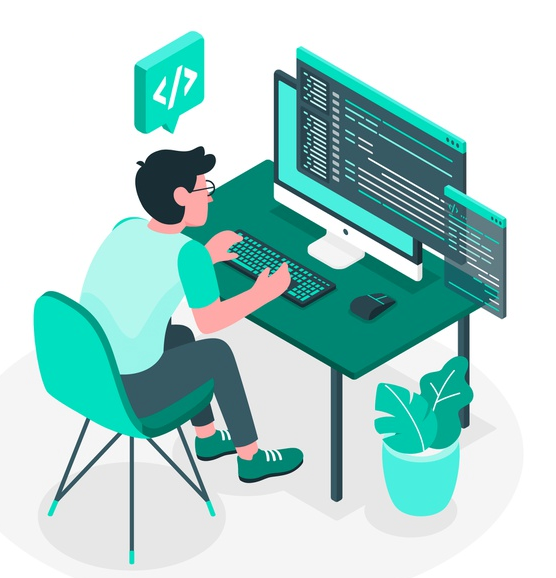
\includegraphics[width=2in]{figs/pkg} 
  \end{figure}
    \column{0.5\textwidth}
     \vspace{1cm}
\begin{itemize}
  \fs
  \item \textcolor{blue}{open source}
  \item \textcolor{blue}{freeware}
  \item \textcolor{blue}{shareware}
  \item \textcolor{blue}{network license}
  \item \textcolor{blue}{single user license}
  \item \textcolor{blue}{software as a service (SaaS)}
  \end{itemize}
%  \vspace{-2cm}
  \end{columns}
\end{frame}

\begin{frame}\frametitle{Writing tools}
{\bf WYSIWYG Editors:}\\
\begin{figure}
    \centering
    
\includegraphics[width=4in]{figs/wt} 
\end{figure}
\begin{itemize}
\fs
\item Office packs: Combine word processor, sheets and presentation softwares
\item Cloud based tools are preferred now {\bf eg:} Office 360 \& Google Docs
\item \textcolor{blue}{LibreOffice} is powerful alternative
\end{itemize}
\end{frame}

\begin{frame}\frametitle{Version Control}
  \begin{columns}[T,onlytextwidth]
    \column{0.5\textwidth}
  \begin{figure}
    \centering
    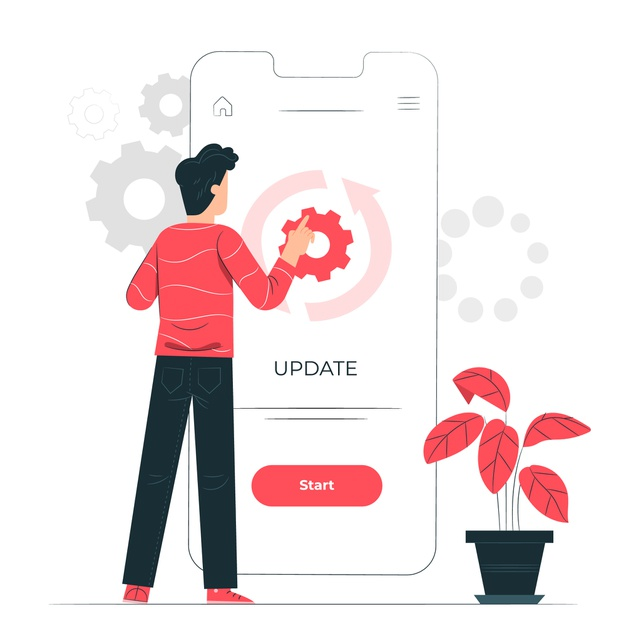
\includegraphics[width=2in]{figs/vc} 
  \end{figure}
    \column{0.5\textwidth}
\fs {\bf Definition:}Version control involves a process of naming and distinguishing between a series of draft documents which lead to a final (or approved) version, which in turn may be subject to further amendments.\\
\begin{itemize}
  \fs
  \item \textcolor{blue}{traceability}
  \item \textcolor{blue}{identifiability}
  \item \textcolor{blue}{clarity}
  \item \textcolor{blue}{reduced duplication}
  \item \textcolor{blue}{reduced errors}
  \end{itemize}
%  \vspace{-2cm}
  \end{columns}
\end{frame}

\begin{frame}\frametitle{Text based processors}
  \begin{columns}[T,onlytextwidth]
    \column{0.5\textwidth}
      \vspace{0.2cm}
  \begin{itemize}
    \fs
	\item text based editors are great for version control
	\item two major languages are: \textcolor{teal}{\LaTeX~ | \texttt{MarkDown}}
	\item \textcolor{blue}{GUI editors:} Gedit | VS Code | Atom
	\item \textcolor{blue}{CLI editors:} nano | vim | emacs
	\item \textcolor{blue}{standalone packages:} Kile | latezila | typora | simplenote
	\item \textcolor{blue}{repos:} Github | Bitbucket | GitLab
  \end{itemize}
  \column{0.5\textwidth}
        \vspace{0.5cm}
  \begin{figure}
    \centering
    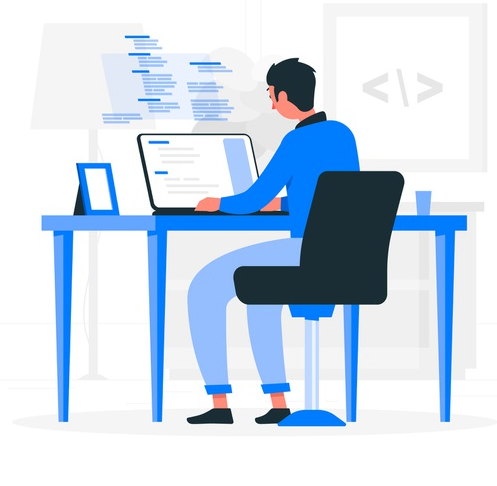
\includegraphics[width=2in]{figs/code} 
  \end{figure}
  \end{columns}
\end{frame}

\begin{frame}\frametitle{Graphing Packages}
  \begin{columns}[T,onlytextwidth]
    \column{0.5\textwidth}
              \vspace{1cm}
  \begin{figure}
    \centering
    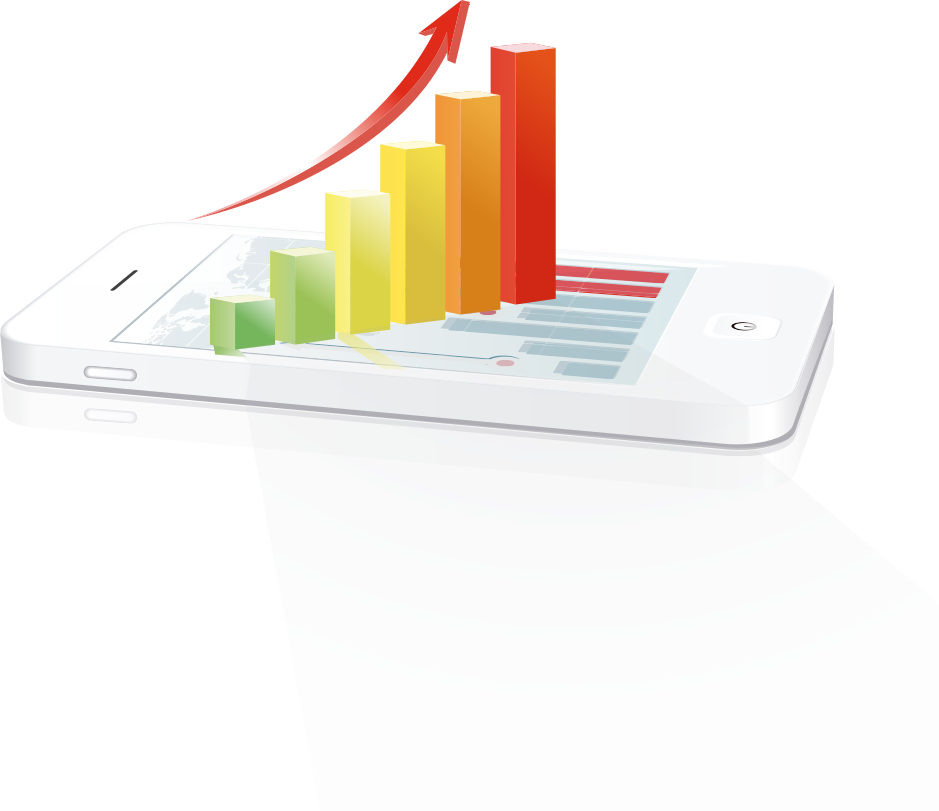
\includegraphics[width=2in]{figs/gps} 
  \end{figure}
    \column{0.5\textwidth}
          \vspace{1cm}
  \begin{itemize}
  \fs
	\item \textcolor{blue}{GUI packages:} Origin Pro | SciDaVis | Kst | Grace
	\item \textcolor{blue}{CLI editors:} gnuplot | KMplot
	\item \textcolor{blue}{Note:} check line densities in MS EXcel
	\item \textcolor{blue}{others:} XYplot
	\end{itemize}
  \vspace{-2cm}
  \end{columns}
\end{frame}

\begin{frame}\frametitle{Simulations}
  \begin{columns}[T,onlytextwidth]
    \column{0.5\textwidth}
      \vspace{1cm}
  \begin{itemize}
    \fs
	\item \textcolor{blue}{MatLab | Octave | SciLab}
	\item \textcolor{blue}{Mathematica | SageMath | Maxima}
	\item \textcolor{purple}{R | GoLang | Python | Julia}
	\item \textcolor{blue}{Always check:} stackexchange | stackoverflow
	\item {\it Note on:} IPython and Jupyter notebook
  \end{itemize}
  \column{0.5\textwidth}
        \vspace{0.5cm}
              \vspace{-0.5cm}
  \begin{figure}
    \centering
    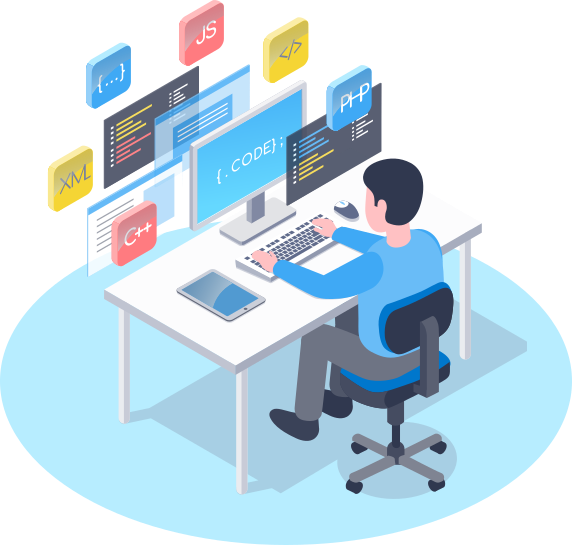
\includegraphics[width=2in]{figs/pgm} 
  \end{figure}
  \end{columns}
\end{frame}

\begin{frame}\frametitle{Images \& drawings}
  \begin{columns}[T,onlytextwidth]
    \column{0.5\textwidth}
  \begin{figure}
    \centering
    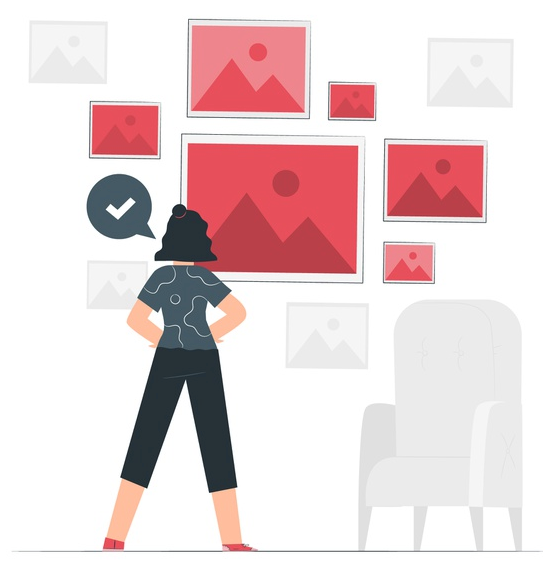
\includegraphics[width=2in]{figs/img} 
  \end{figure}
    \column{0.5\textwidth}
          \vspace{1cm}
  \begin{itemize}
  \fs
	\item \textcolor{blue}{Images:} Photoshop | GIMP
	\item \textcolor{blue}{Drawings:} TGIF | Illustrator | InkScape | CorelDraw
	\item \textcolor{blue}{3D:} Maya | Blender | Google Sketch | LightWave
	\item \textcolor{blue}{others:} MS Publisher | LibreOffice Draw
	\end{itemize}
  \vspace{-2cm}
  \end{columns}
\end{frame}

\begin{frame}\frametitle{Chemical drawings \& simulations}
  \begin{columns}[T,onlytextwidth]
    \column{0.5\textwidth}
      \vspace{1cm}
  \begin{itemize}
    \fs
	\item \textcolor{blue}{Sketch:} ChemDraw | ChemSketch | MarvinSketch
	\item \textcolor{blue}{Visualization:} Avogadro | Gabedit | Pymol | Mercury
	\item \textcolor{purple}{Simulation:} Gaussian | ORCA | MOPAC
	\item \textcolor{blue}{Structure:} IUPAC | COD | RCSB-PDB
  \end{itemize}
  \column{0.5\textwidth}
        \vspace{0.5cm}
              \vspace{-0.5cm}
  \begin{figure}
    \centering
    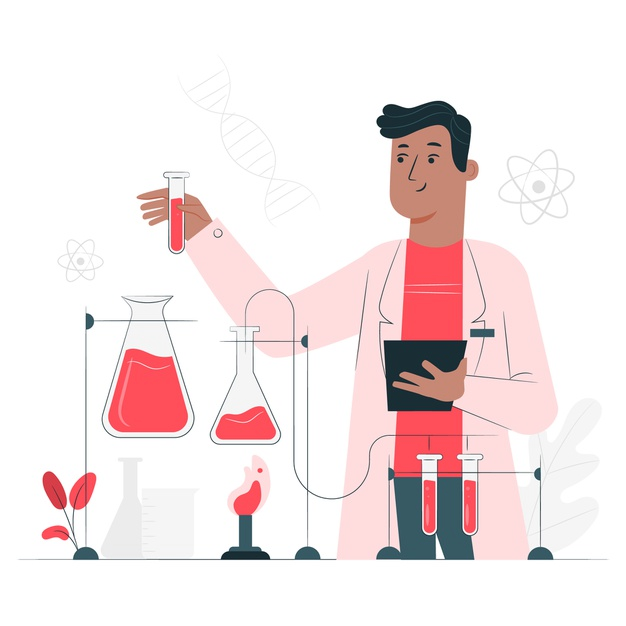
\includegraphics[width=2in]{figs/che} 
  \end{figure}
  \end{columns}
\end{frame}

\begin{frame}\frametitle{Language tools}
  \begin{columns}[T,onlytextwidth]
    \column{0.5\textwidth}
  \begin{figure}
    \centering
    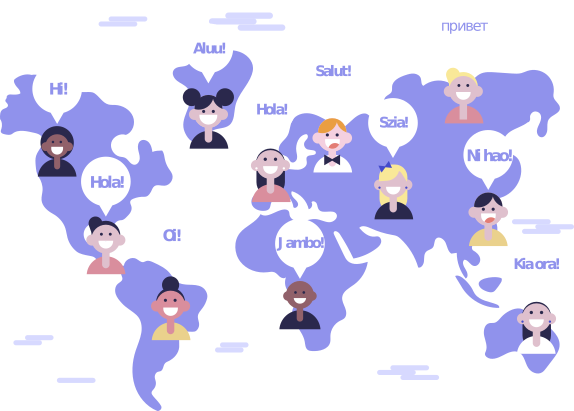
\includegraphics[width=2in]{figs/world} 
  \end{figure}
    \column{0.5\textwidth}
%          \vspace{1cm}
  \begin{itemize}
  \fs
	\item \textcolor{blue}{Grammar:} Built-in tools
	\item \textcolor{blue}{Online tools:} Grammarly | Language Tools | Slickwrite
	\item \textcolor{blue}{Others:} WhiteSmoke | Ginger
	\item \textcolor{purple}{Plagiarism:} Urkund | Prowriting Aid | Paperrater
	\item Good with pyhton? Check github repos for self checkers
	\end{itemize}
  \vspace{-2cm}
  \end{columns}
\end{frame}

\begin{frame}\frametitle{Reference managers}
  \begin{columns}[T,onlytextwidth]
    \column{0.5\textwidth}
      \vspace{1.5cm}
  \begin{itemize}
    \fs
	\item \textcolor{blue}{Mendeley | Zotero | EndNote}
	\item \textcolor{teal}{Google Scholar | Scite.ai}
	\item \textcolor{purple}{Bookmarks:} Raindrop | Pocket
	\item \textcolor{blue}{Paperpile | Citavi | JabRef}
  \end{itemize}
  \column{0.5\textwidth}
        \vspace{0.5cm}
              \vspace{-0.5cm}
  \begin{figure}
    \centering
    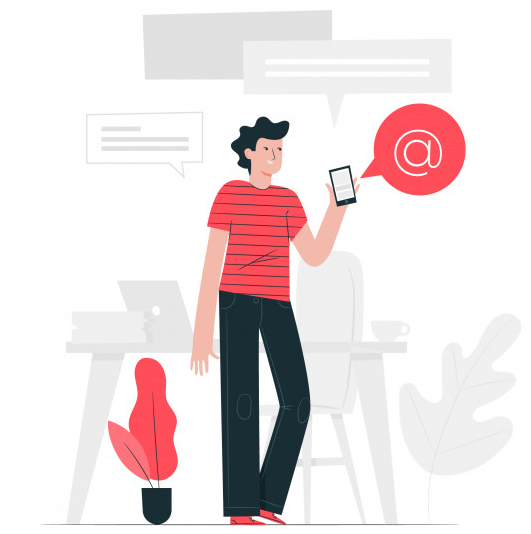
\includegraphics[width=2in]{figs/ref} 
  \end{figure}
  \end{columns}
\end{frame}

\begin{frame}\frametitle{Preprints \& journal selectors}
  \begin{columns}[T,onlytextwidth]
    \column{0.5\textwidth}
      \vspace{0.5cm}
      {\fs \bf List of preprint servers:}\\
  \begin{itemize}
    \fs
    	\item \textcolor{red}{\it Difference between preprint \& journal article}
	\item \textcolor{blue}{Arxhive | Zenodo}
	\item \textcolor{blue}{ChinaXiv | INA-Rxiv}
	\item \textcolor{teal}{Chemarxiv | Bioarxiv | Engrxiv}
	\item \textcolor{blue}{OSF Preprints | Preprints.org}
  \end{itemize}
        {\fs {\bf Journal selectors:} Edanz | Cofactor }
          \column{0.5\textwidth}
              \vspace{-0.5cm}
  \begin{figure}
    \centering
    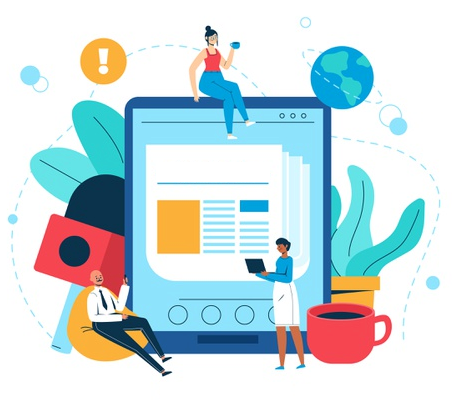
\includegraphics[width=2in]{figs/jnl} 
  \end{figure}
  \end{columns}
\end{frame}

\section{Summary}

\begin{frame}\frametitle{Take home message}
  \begin{columns}[T,onlytextwidth]
    \column{0.5\textwidth}
  \begin{figure}
    \centering
    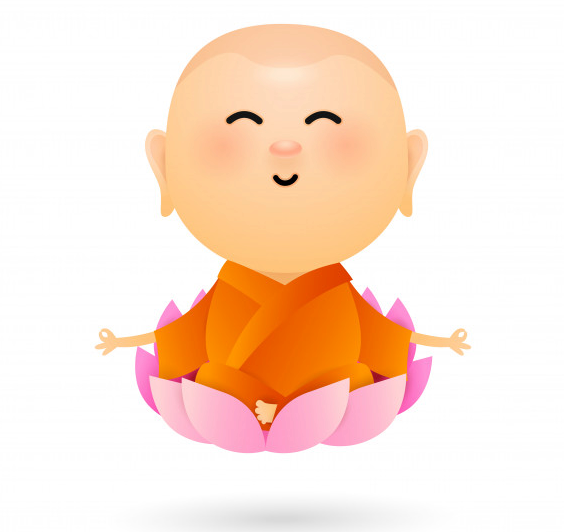
\includegraphics[width=2in]{figs/bud} 
  \end{figure}
    \column{0.5\textwidth}
          \vspace{1.5cm}
  \begin{itemize}
  \fs
	\item \textcolor{blue}{Ethics: ground rules}
	\item \textcolor{blue}{When \& what to publish?}
	\item \textcolor{purple}{Language and formatting}
	\item \textcolor{blue}{Which tool to choose?}
	\end{itemize}
  \vspace{-2cm}
  \end{columns}
\end{frame}

\begin{frame}\frametitle{Selected Read}
  \begin{enumerate}
    \fs
	\item Barrass, R. \textcolor{blue}{Scientists Must Write: A Guide to Better Writing for Scientists, Engineers, and Students,} 2nd ed.; Routledge: London, 2002.
	\item Day, R. A. \textcolor{blue}{Scientific English: A Guide for Scientists and Other Professionals,} 2nd ed.; Oryx Press: Phoenix, AZ, 1995.
	\item Zinsser, W. \textcolor{blue}{Writing To Learn}; Collins: New York, 1993
	\item \textcolor{blue}{AIP Style Manual}, 4th ed.; American Institute of Physics: New York, 1990
	\item \textcolor{blue}{ACS Style Guide}, 3rd ed.; American Chemical Society: Washington DC, 2006
  \end{enumerate}
\end{frame}

\begin{frame}\frametitle{Acknowledgements}
\begin{itemize}
\fs
\item {\bf \textcolor{blue}{Dr. T. Kanagasekaran}}, \textcolor{purple}{IISER Tirupati} -- for corrections \& improvement
\item {\bf \textcolor{blue}{Dr. K. Suresh}}, \textcolor{purple}{University of Delhi} -- for content suggestions \& perspectives
\item {\bf \textcolor{blue}{Dr. R. Jothimurugan}}, \textcolor{purple}{GTN Arts \& Sci. Colg, Dindigul} -- for delivering ideas
\item {\bf \textcolor{blue}{Dr. Shika Kumari}}, \textcolor{purple}{JNU, Delhi} -- for overall review
\item {\bf \textcolor{blue}{Dr. Ganesh}}, \textcolor{purple}{SKCT, Coimbatore} -- for coordinating \& audience based content management
\end{itemize}
\end{frame}

\begingroup
\setbeamercolor{background canvas}{bg=sthlmDarkGrey}
\begin{frame}[plain,containsverbatim]
\begin{figure}
\centering

\includegraphics[width=2in]{figs/alt}
\end{figure}
\end{frame}
\endgroup

\end{document}
